\documentclass[a4paper,10pt]{article}
\usepackage[utf8]{inputenc}
\usepackage{graphicx}
\usepackage{float}
\usepackage[margin=0.7in]{geometry}

%opening
\title{Parallel and Concurrent Programming\\
Course Project\\
Wait-free Extensible Hashmaps \\
using Multi-level Arrays}
\author{Agam Agarwal \hspace{0.5cm} CS12B1003\\
Rakshit Singla \hspace{0.5cm} CS12B1029}


\begin{document}

\maketitle
\pagebreak
\tableofcontents
\pagebreak
\section{Problem Statement}
The project presents the implementation of a wait-free hash map.
This data structure allows a large number of threads to concurrently
\verb put, \verb get, and \verb remove  values.

\subsection{Wait-Freedom}
Wait-freedom means that all threads make progress in a finite amount of time.
This is opposed to the traditional blocking implementations of shared
data structures which suffer from the negative impact of deadlock
and related correctness and performance issues.
\subsection{CAS Operation}
This design is portable because we only use the Compare-and-Swap
atomic operation which is provided by hardwares.

\section{Wait Free extensible Hashmaps}
\begin{figure}[h!]
  \begin{center}
 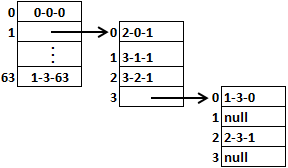
\includegraphics{WFEexample}
  \end{center}
 \caption{An example of data stored in the hash map (values not
shown)}
\end{figure}
In this implementation of hashmap, the \verb {key,value}  pairs are stored in multilevel arrays.
The \verb key  is hashed and then cut into chunks of fixed sizes. These fixed size chunks are used 
to decide the level in the multilevel array.

In a multi-level array each \verb Node  is either a \verb DataNode  or an \verb ArrayNode  .
\begin{itemize}
 \item \verb DataNode  : It contains \verb {key,hash,value} . 
 \item \verb ArrayNode  : It contains pointer to an array of nodes which are accessible depending on the next chunk of the \verb hash  . 
\end{itemize}

In the above example, the second level contains nodes with hashes $3-2-1$ and $3-1-1$. As we can see, they are pointed to
by the \verb ArrayNode  in the $1^{th}$ slot of the previous level. In the second level the key $3-2-1$ is put in the $2^{th}$ slot
because the $2^{nd}$ last chunk in the \verb hash  is the value $2$. Similarly, the key $3-1-1$ is put in the $1^{th}$ slot in 
the second level.

\section{Lock-Based Extensible Hashmap}
We also implemented a lock based extensible hashmap using multilevel arrays. In this approach, the correctness is guaranteed as
every thread acquires the \verb lock  before doing any operation (put, get, remove) on the hashmap.
This implementation was done to compare the performance of the Wait-free hashmap which the paper claims to be atleast 5X faster
than the lock based methods.

\section{Testing}
For testing, we spawn number of threads to do the three operations and then calculate the time taken by these threads to
complete the operations.\\

\begin{tabular}{|l|c|}
\hline
Number of threads per operation (\verb put,get,remove ) & $5,10,15,...,40$ \\ \hline
Number of operations per thread & $20$ \\ \hline
Sleep time & Exponention distribution with mean $ = 10 \mu s$ \\ \hline
\end{tabular}

\section{Results and Comparisons}
To compare the performance of these implementations we measure the average time for each operation for both the 
implementations over a varying number of threads. The results of these comparisons are given below -
\begin{figure}[H]
 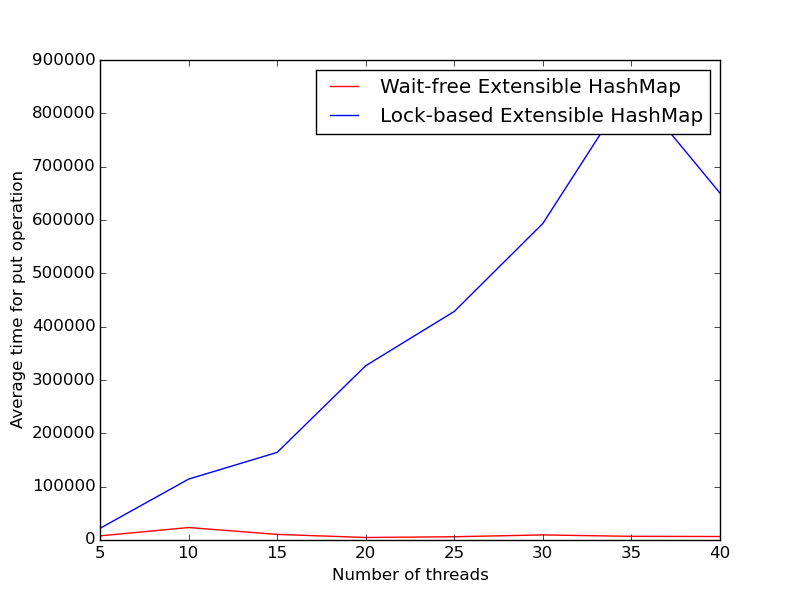
\includegraphics[width=\linewidth]{put.png}
 \caption{Average time of put operation(in $\mu$s)}
\end{figure}

\begin{figure}[H]
 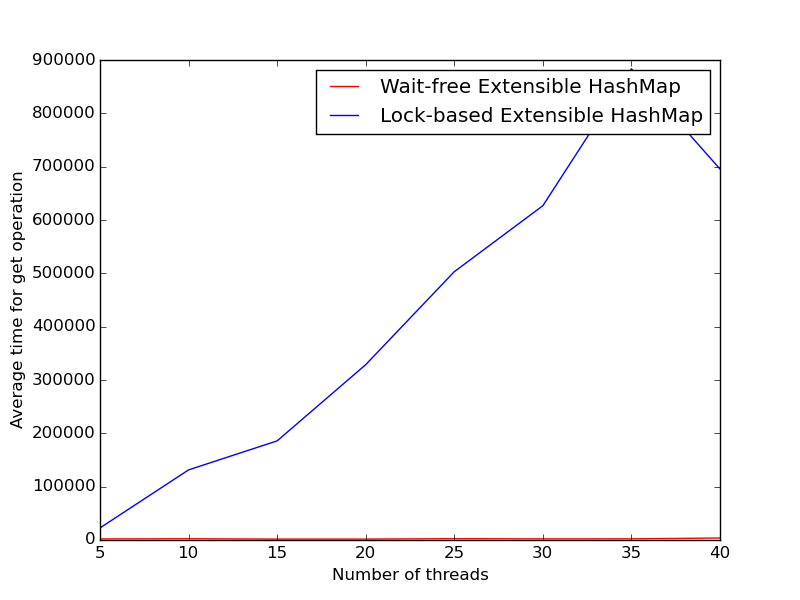
\includegraphics[width=\linewidth]{get.png}
 \caption{Average time of get operation(in $\mu$s)}
\end{figure}

\begin{figure}[H]
 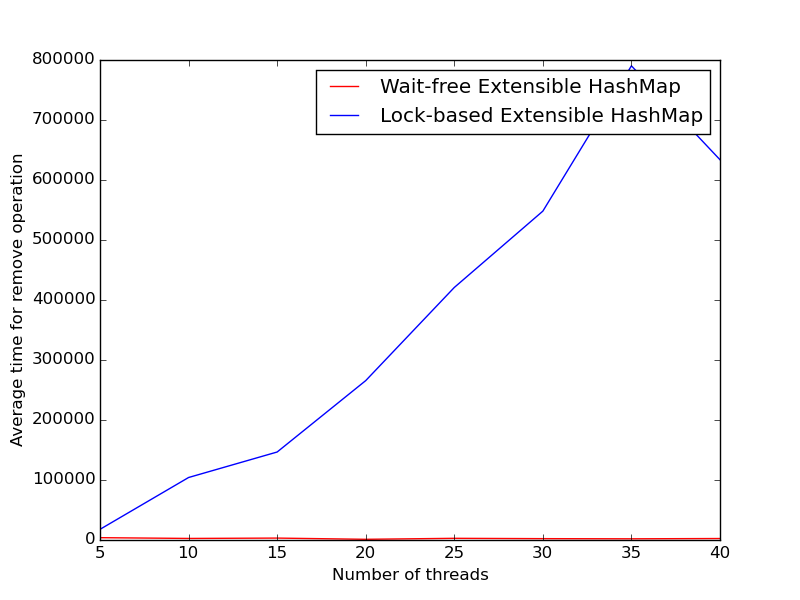
\includegraphics[width=\linewidth]{remove.png}
 \caption{Average time of remove operation (in $\mu$s)}
\end{figure}

\section{Conclusions}
As we can see from the graphs, the results for the Wait-free implementation are much better than that of
lock-based implementation (much more than 5X as claimed by the paper). This is as expected because in wait-free methods
there are no locks and thus the threads do get blocked when some other thread is already accessing the hashmap.
\section{References}
\begin{enumerate}
 \item Feldman, Steven, Pierre LaBorde, Damian Dechev. "Concurrent multi-level arrays: Wait-free extensible hash maps."
 \textit{Embedded Computer Systems: Architectures, Modeling, and Simulation (SAMOS XIII), 2013 International Conference on. IEEE, 2013.}
\end{enumerate}

\end{document}
